\documentclass[aspectratio=169, table]{beamer}
\usepackage[utf8]{inputenc}
\usepackage{xcolor}

\usepackage{multicol}
\usepackage{booktabs}
\usepackage{arydshln}
\usepackage[abs]{overpic}
\usepackage{tikz}
\usetikzlibrary{fadings}
%\usepackage{enumitem}
%\usepackage[table]{xcolor} 

\usepackage{empheq}

 \definecolor{redp}{rgb}{0.78, 0.03, 0.08}
\definecolor{greenp}{rgb}{0.0, 0.51, 0.5}
\definecolor{yellowp}{rgb}{0.59, 0.44, 0.09}
\definecolor{greencol}{rgb}{0.0,0.4,0.0}
\definecolor{fcolor}{rgb}{0.8, 0.4, 0.0}

\newcommand{\enb}[1]{\textcolor{poliblue1}{\textbf{#1}}}
\newcommand{\eno}[1]{\textcolor{orange}{\textbf{#1}}}
\definecolor{softblue}{cmyk}{.2, .1, .1, .2}
\newcommand{\soft}[1]{\textcolor{softblue}{#1}}

\title{Optimistic Policy Optimization via Multiple Importance Sampling}
\date[AAA]{\vspace{0.2cm} \\ \small{ 11th June 2019 \\ Thirty-sixth International Conference on Machine Learning, Long Beach, CA, {USA}}}
\author[M. Papini]{\textbf{Matteo Papini} \quad Alberto Maria Metelli\\
						\small{Lorenzo Lupo \quad Marcello Restelli}}

\usetheme{polimithx}
\usetikzlibrary{calc}

\usepackage[customcolors,shade]{hf-tikz}

%%%%%%%%%%%%%%%%%%%%%%%%%% BIBLIOGRAPHY
\usepackage{natbib}
\bibliographystyle{apalike}
% make bibliography entries smaller
\renewcommand\bibfont{\scriptsize}
% If you have more than one page of references, you want to tell beamer
% to put the continuation section label from the second slide onwards
\setbeamertemplate{frametitle continuation}[from second]

%CUSTOM COMMANDS

\usepackage[many]{tcolorbox}
\usetikzlibrary{decorations.pathreplacing}
\usetikzlibrary{arrows,shapes}
\usetikzlibrary{positioning}

\usepackage{mymacros}

\begin{document}

\setbeamertemplate{caption}{\raggedright\insertcaption\par}

\begin{frame}
\titlepage
\end{frame}

\begin{frame} 
\frametitle{Policy Optimization} 
\begin{itemize}
	\item \enb{Parameter space} $\Theta \subseteq \Reals^d$
	\item A parametric \enb{policy} for each $\vtheta\in\Theta$
	\item Each inducing a distribution $p_{\vtheta}$ over \enb{trajectories}
	\item A \enb{return} $R(\tau)$ for every trajectory $\tau$
	\vfill
	\begin{center}
	\Large \enb{Goal:} $\max\limits_{\vtheta\in\Theta} J(\vtheta) = \Exp_{\tau\sim p_{\vtheta}}\left[R(\tau)\right]$
	\end{center}
	\vfill
	\item On-line, iterative optimization
\end{itemize}
\end{frame}

\begin{frame} 
\frametitle{Exploration in Policy Optimization} 
\begin{itemize}
	\item \enb{Exploration-exploitation} trade-off
	\item \eno{Problem:} the underlying Markov process is often \eno{continuous}
	\item \enb{Undirected} exploration: entropy bonus~\citep{haarnoja2018soft}
	\item \enb{Directed} exploration: pseudo-counts~\citep{bellemare2016unifying}
	\vfill
	\centering
	{\Large\eno{Lack} of theoretical guarantees}
\end{itemize}
\end{frame}

\begin{frame} 
\frametitle{Policy Optimization as a MAB } 
\begin{itemize}
	\item \enb{Arms:} parameters $\vtheta$
	\item \enb{Payoff:} expected return $J(\vtheta)$
	\item \eno{Continuous MAB}~\citep{kleinberg2013bandits}: we \emph{need} structure
\end{itemize}
\vfill
\centering
{\Large\enb{Arm correlation}~\citep{pandey2007multi} through trajectory distributions}

\end{frame}

\begin{frame} 
\frametitle{OPTIMIST} 
\begin{itemize}
	\item A \enb{UCB-like} index~\citep{lai1985asymptotically}:
	\begin{align*}
	\large
		B_t(\vtheta) =
		\underbrace{\wc{\mu}_t(\vtheta)}_{\substack{\textbf{ESTIMATE:}\\\\\text{a \eno{truncated} \enb{multiple}}\\ \text{ importance sampling estimator~\cite{veach_optimally_1995,bubeck2013bandits}}}}
		+
		\underbrace{R_{\max}\left(\sqrt{2}+\frac{4}{3}\right)
		\sqrt{\frac{d_{2}(p_{\vtheta}\|\Phi_{t})\log\frac{1}{\delta_t}}{t}}}_{\substack{\textbf{EXPLORATION BONUS:}\\\\\text{\enb{distributional} distance} \\ \text{from previous arms}}}
	\end{align*}
	\item Select $\vtheta_t = \arg\max\limits_{\vtheta\in\Theta} B_t(\vtheta)$
\end{itemize}
\end{frame}

\begin{frame} 
\frametitle{Sublinear Regret} 
\begin{itemize}
	\item Recall $\mathop{Regret}(T) = \sum_{t=0}^T J(\vtheta^*) - J(\vtheta_t)$
	\vfill
	\item Consider a \enb{compact}, $d$-dimensional parameter space $\Theta$
	\vfill
	\item Under \enb{mild assumptions} on the policy class, with high probability:
	\Large
	\begin{align*}
		\mathop{Regret}(T) = \wt{\mathcal{O}}\left(\sqrt{dT}\right)
	\end{align*}
	
\end{itemize}
\end{frame}

\begin{frame} 
\frametitle{Empirical Results} 
\begin{columns}
	\begin{column}{.5\textwidth}
		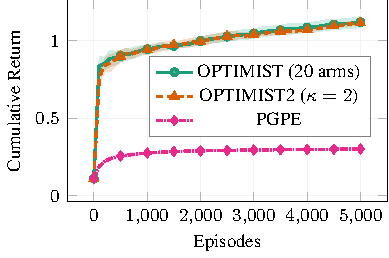
\includegraphics[]{river.pdf}
	\end{column}
	\begin{column}{.5\textwidth}
		\eno{Caveats}
		\begin{itemize}
			\item Easy implementation only for parameter-based exploration
			\item Difficult optimization $\implies$ discretization
			\item ...
		\end{itemize}
	\end{column}
\end{columns}
\end{frame}

\begin{frame}[plain]
%\frametitle{Thanks} 
\begin{center}
	\huge{\enb{Thank You for Your Attention!}}
\end{center}

\begin{minipage}[]{.5\paperwidth}
	\begin{itemize}
		\item Poster \textbf{\#103}
		\item Code: \url{github.com/WolfLo/optimist}
		\item Contact: matteo.papini@polimi.it
		\item Web page: \url{t3p.github.io/icml19} 
	\end{itemize}
\end{minipage}
\hspace{2cm}%
\begin{minipage}[]{.2\paperwidth}
	
\includegraphics[width=\textwidth]{qr.png}
\end{minipage}
\end{frame}


%%%%%%%%%%%%%%%%%%%%%%%%%%%%%%%%%%%%%%%%%%%%%%%%%%%%%%%%%%%%%%%%%%%%%%%%%%%%%%%%%%%%%%%%%
\begin{frame}[allowframebreaks,fragile]
\frametitle{References}
\bibliographystyle{abbrv}
\bibliography{../biblio.bib}
\end{frame}
%%%%%%%%%%%%%%%%%%%%%%%%%%%%%%%%%%%%%%%%%%%%%%%%%%%%%%%%%%%%%%%%%%%%%%%%%%%%%%%%%%%%%%%%%

%%Backup Slides


\end{document}
